\documentclass[12pt]{article}
\usepackage{pgf, tikz}
\usepackage{amsmath, amsfonts, amssymb, graphicx}
\usepackage{float}
\usepackage{subfig}
\usepackage[utf8]{inputenc}
\usepackage[spanish]{babel}
\usepackage{amsthm}
\usepackage{caption}

\setlength{\textheight}{23cm} \setlength{\evensidemargin}{0cm}
\setlength{\oddsidemargin}{-.5cm} \setlength{\topmargin}{-3cm}
\setlength{\textwidth}{17.5cm} \setlength{\parskip}{.2cm}


%opening

\begin{document}
	\begin{picture}(80, 80)
	\put(170,0){\hbox{
\includegraphics[scale=0.6]{cimat_logo.png}}}
	\end{picture}
	
	\begin{center}
		\begin{huge}
			Centro de Investigación en Matemáticas, A.C.
		\end{huge}
	\end{center}

	\begin{center}
		\begin{large}
			Descripción tarea 10 - Métodos numéricos
		\end{large}
	\end{center}
	
	\begin{center}
		\textbf{Erick Salvador Alvarez Valencia}
	\end{center}

	\begin{center}
		5 de Noviembre de 2017
	\end{center}



%\maketitle

%\tableofcontents

\section{Introducción}
En el presente reporte se describirán los resultados de dos métodos empleados en la tarea 10 para la interpolación polinomial, el primero consiste en resolver un problema de minimización empleando elemento finito y el segundo consiste en realizar el desarrollo de un spline cúbico para la interpolación. Se presentarán los resultados de las ejecuciones así como algunas gráficas formadas a través de ellos.

\section{Problema de minimización}

\subsection{Descripción}
En este ejercicio se presentó un problema de minimización de la siguiente función:

$$min_{\phi_0,\phi_1,...,\phi_n \sum_{i=1}^{m}[\phi(x_i)-y_i]^2+\lambda \int_{0}^{10}(\phi')^2}$$

Para lo cual se utilizó la técnica de elemento finito, con ella se hizo una discretización para poder construir un sistema de ecuaciones tridiagonal y así encontrar el arreglo de $\phi_i$. Al final el programa se probó con varios valores de $\lambda$ los cuales generan una penalización en la parte de suavidad del polinomio interpolador.

\subsection{Ejemplo de ejecución}
A continuación se mostrará el resultado de la ejecución del programa usando dos conjuntos de datos distintos y a su vez valores de $\lambda$ distintos.

\begin{figure}[H]
	\centering
	\subfloat[][Figura 1. Conjunto de datos 1, lambda = 0.1.]{
		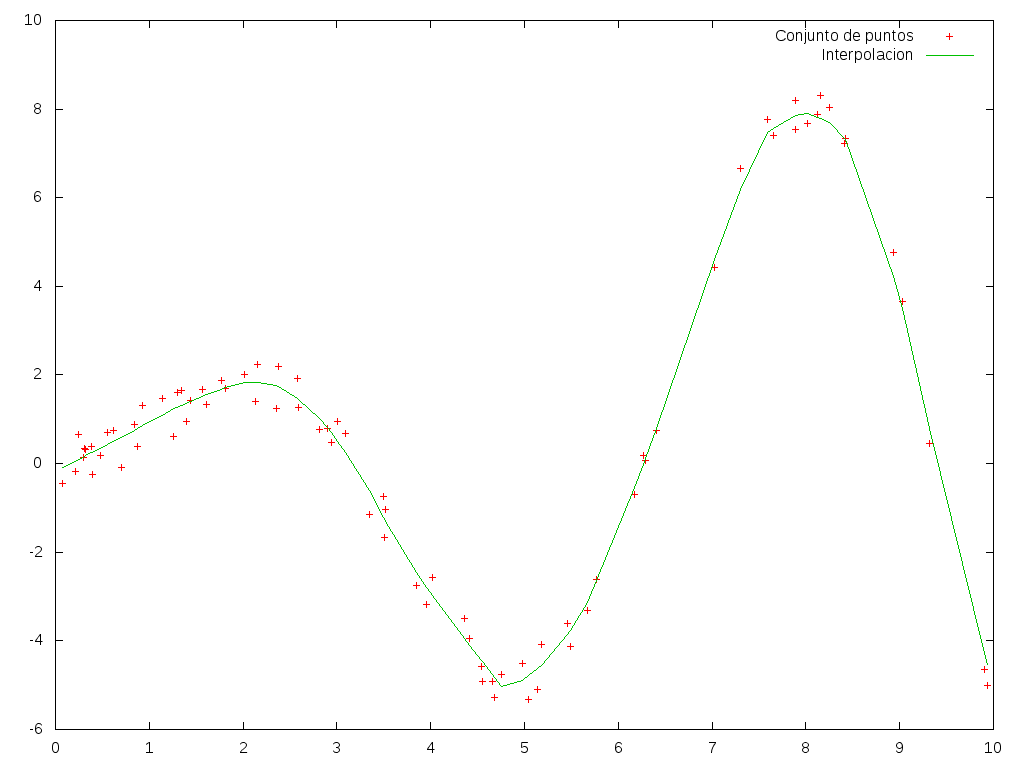
\includegraphics[scale=0.4]{Grafica1.png}
	}\hfill
\end{figure}

\begin{figure}[H]
	\centering
	\subfloat[][Figura 2. Conjunto de datos 1, lambda = 10.]{
		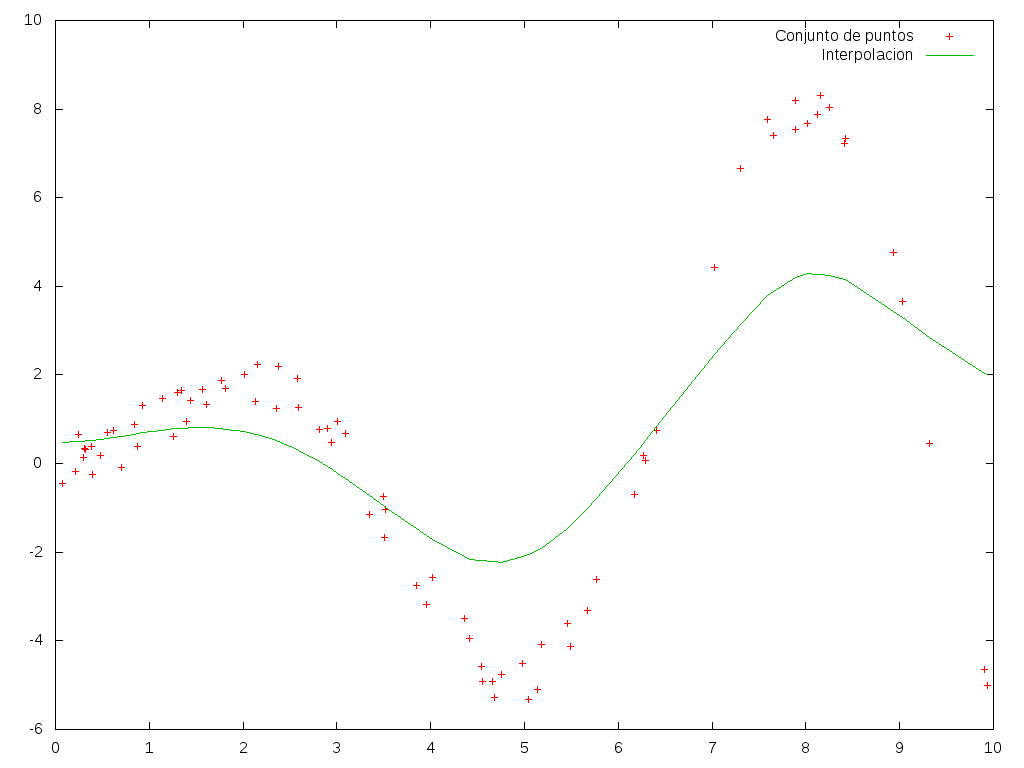
\includegraphics[scale=0.4]{Grafica11.png}
	}\hfill
\end{figure}

En las Figuras 1 y 2. podemos observar la ejecución del mismo algoritmo pero con una variación en el parámetro lambda que genera una gran penalización en el polinomio interpolador, ya que para el promer lambda dado se genera una muy buena interpolación y para el otro hay muchas diferencias en la nube de puntos con respecto a la curva.

\begin{figure}[H]
	\centering
	\subfloat[][Figura 3. Conjunto de datos 2, lambda = 0.1.]{
		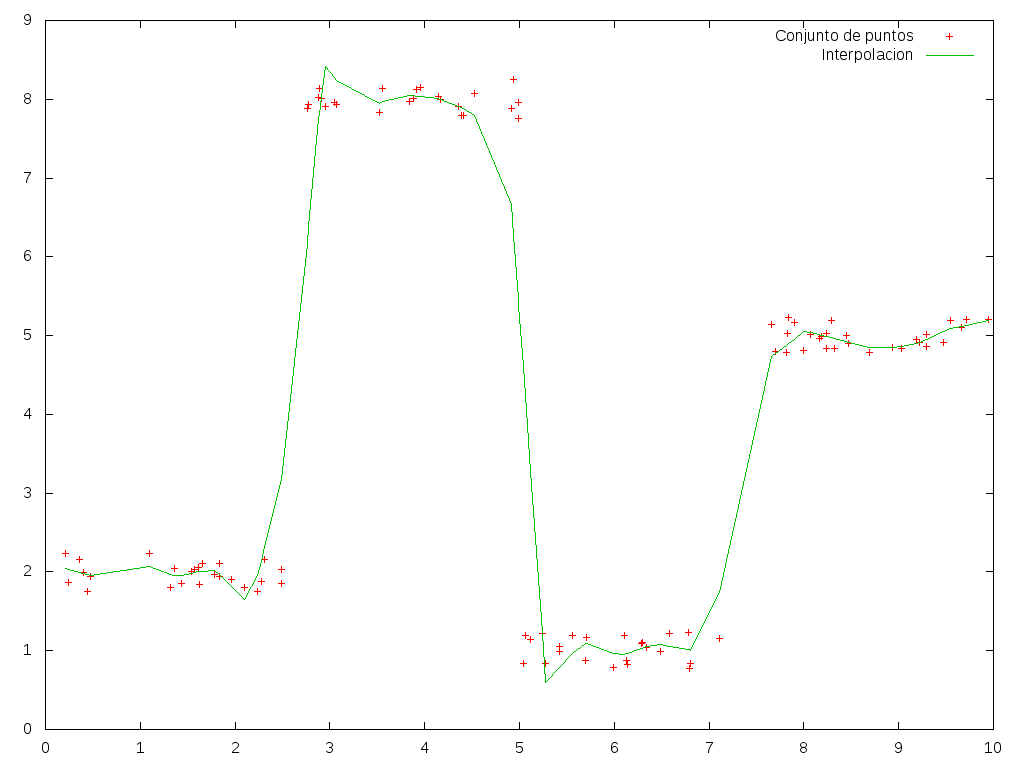
\includegraphics[scale=0.4]{Grafica2.png}
	}\hfill
\end{figure}

\begin{figure}[H]
	\centering
	\subfloat[][Figura 4. Conjunto de datos 2, lambda = 10.]{
		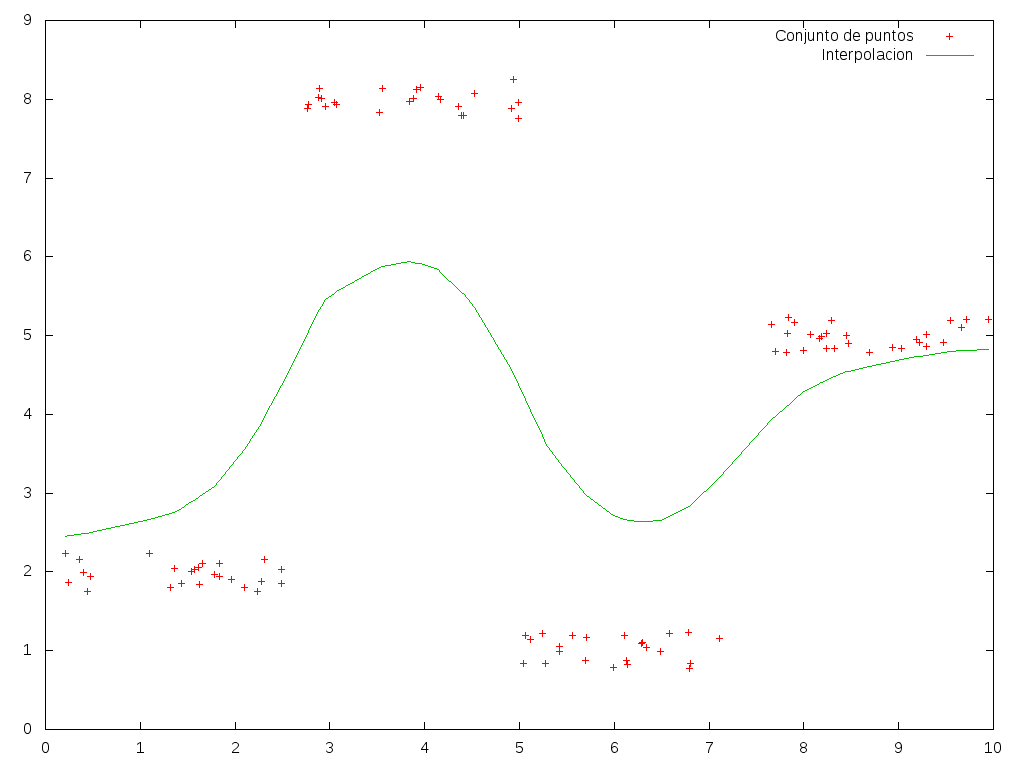
\includegraphics[scale=0.4]{Grafica21.png}
	}\hfill
\end{figure}

Al igual que en el caso anterior, se ejecutó el programa con dos diferentes lambdas para ver la penalización provocada por las mismas. En las Figuras 3 y 4. se puede apreciar la diferencia de la interpolación provocada por un lambda de 0.1 y otro de 10.

\subsection{Observaciones}
Cabe destacar que en el código se definió la función $phi(x)$ como se describe en la presentación de la clase usando las funciones $N_k$ y $N_{k+1}$ y no usando la delta de Kronecker.

\section{Splines}
\subsection{Descripción}
Para este ejercicio se dieron un conjunto de puntos y se propuso un spline cúbico que los interpolara, para ello se analizó el desgloce propuesto en el paper de la clase de Splines y se logró definir un sistema tridiagonal que al resolverlo nos daría el arreglo de $M_i$ el cual serviría para generar los splines $S(x_i)$.

\subsection{Ejemplo de ejecución}
A continuación se mostrarán los resultados de la ejecución del programa con dos conjuntos distintos de puntos.

\begin{figure}[H]
	\centering
	\subfloat[][Figura 4. Conjunto de datos 1.]{
		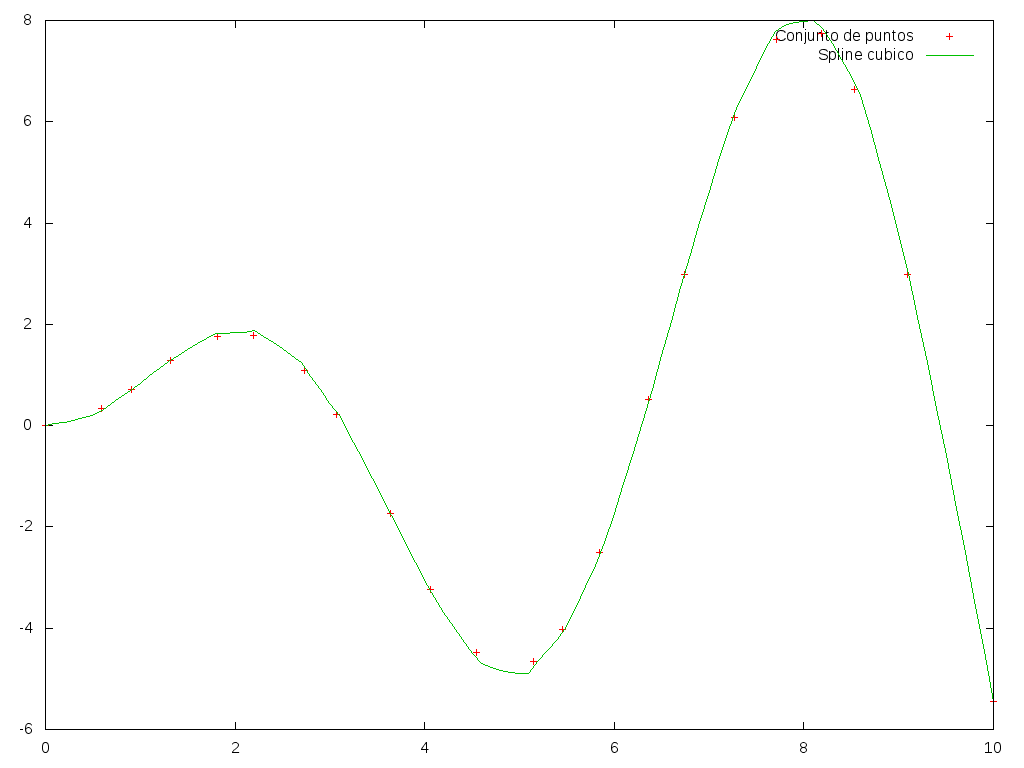
\includegraphics[scale=0.4]{Grafica3.png}
	}\hfill
\end{figure}

\begin{figure}[H]
	\centering
	\subfloat[][Figura 5. Conjunto de datos 2.]{
		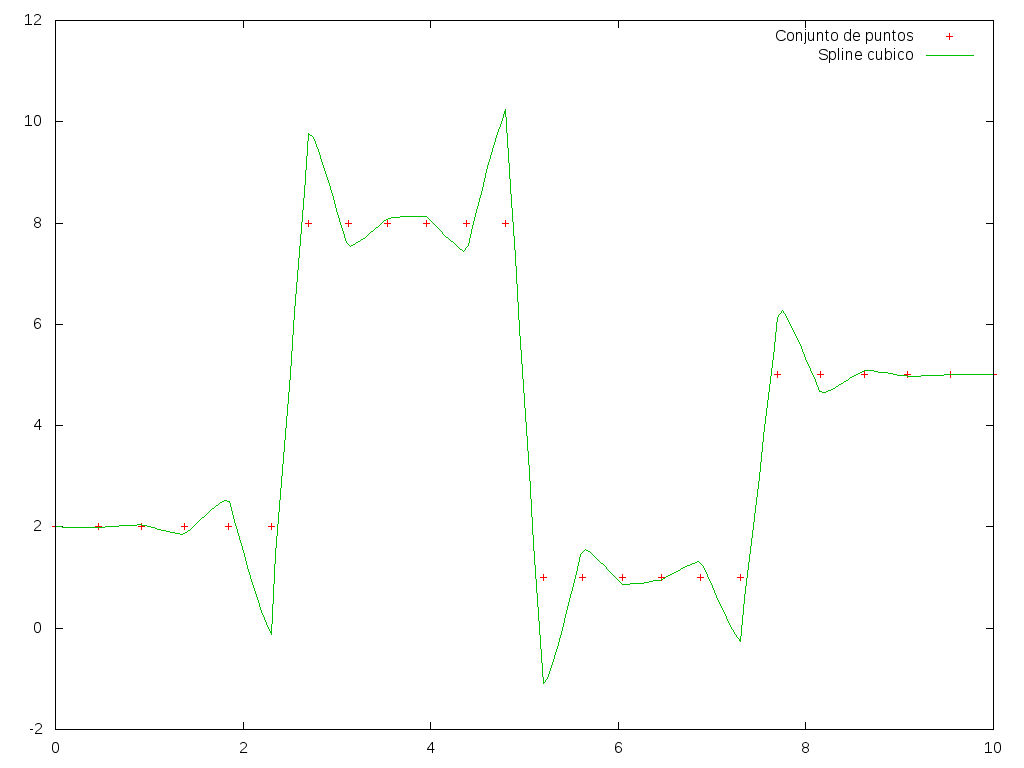
\includegraphics[scale=0.4]{Grafica4.png}
	}\hfill
\end{figure}

Se puede ver en las gráficas anteriores que los conjuntos de puntos fueron interpolados por los splines definidos a pares. Aunque en el conjunto dos se pueden notar unos picos y valles tal vez no deseados, esto puede presentarse porque la función está definida a trozos y se genera el genómeno de Gibbs.

\section{Compilación y ejecución}
Para esta tarea, los programas se dividieron en tres carpetas, mediante las cuales se encuentran los archivos del código y los de prueba, hay que mencionar que para cada programa se usará la misma forma de compilar, por lo que solo es necesario describir los pasos una vez.\\

\textbf{Para compilar:} En la carpeta encontraremos los archivos $.c$ y $.h$ con los que se podrá compilar el ejecutable. De la misma forma, en conjunto con los archivos anteriores, también podremos encontrar un Makefile para, en caso de encontrarse en linux, compilar de manera sencilla.

\begin{enumerate}
	\item \textbf{Compilar usando Makefile:} En la terminal, nos colocamos en el directorio donde se encuentre el programa, y ejecutamos el comando $make$, automáticamente se realizará la compilación y se generará el ejecutable. El Makefile también contiene el comando $make\ clean$ el cual limpiará los archivos generados por la compilación, incluyendo el ejecutable.
	\item \textbf{Compilar directamente:} De la misma forma, podemos compilar directamente usando los siguientes comandos (en terminal):
	\begin{itemize}
		\item gcc -c main.c -o obj/main.o
		\item gcc -c memo.c -o obj/memo.o
		\item gcc -c reader.c -o obj/reader.o
		\item gcc -c matriz\_vector.c -o obj/matriz\_vector.o
		\item gcc -c met\_num.c -o obj/met\_num.o
		\item gcc -o main obj/main.o obj/memo.o obj/reader.o obj/matriz\_vector.o obj/met\_num.o\ -lm
	\end{itemize}
\end{enumerate}

\textbf{Para ejecutar (programa 1):} Únicamente debemos de usar el comando $./main$ para ejecutar el programa en consola, este recibe los siguientes argumentos:
\begin{itemize}
	\item \textbf{Un string:} El nombre del archivo binario donde se encuentra la matriz de puntos.
	\item \textbf{Un entero}: El tamaño de la discretización que se generará.
	\item \textbf{Un doble}: El valor $\lambda$ que penalizará la interpolación. 
\end{itemize}

El programa ejecutará generará un archivo de texto el cual contendrá los valores de los puntos del polinomio interpolador.\\

\textbf{Para ejecutar (programa 2):} Únicamente debemos de usar el comando $./main$ para ejecutar el programa en consola, este recibe los siguientes argumentos:
\begin{itemize}
	\item \textbf{Un string:} El nombre del archivo binario donde se encuentra la matriz de puntos.
	\item \textbf{Un entero}: El tamaño de puntos que contendrá el spline. 
\end{itemize}

El programa ejecutará generará un archivo de texto el cual contendrá los valores de los puntos del spline.\\

\end{document}
